\documentclass[journal]{vgtc}                     % final (journal style)
%\documentclass[journal,hideappendix]{vgtc}        % final (journal style) without appendices
%\documentclass[review,journal]{vgtc}              % review (journal style)
%\documentclass[review,journal,hideappendix]{vgtc} % review (journal style)
%\documentclass[widereview]{vgtc}                  % wide-spaced review
%\documentclass[preprint,journal]{vgtc}            % preprint (journal style)


%% Uncomment one of the lines above depending on where your paper is
%% in the conference process. ``review'' and ``widereview'' are for review
%% submission, ``preprint'' is for pre-publication in an open access repository,
%% and the final version doesn't use a specific qualifier.

%% If you are submitting a paper to a conference for review with a double
%% blind reviewing process, please use one of the ``review'' options and replace the value ``0'' below with your
%% OnlineID. Otherwise, you may safely leave it at ``0''.
\onlineid{0}

%% In preprint mode you may define your own headline. If not, the default IEEE copyright message will appear in preprint mode.
%\preprinttext{To appear in IEEE Transactions on Visualization and Computer Graphics.}

%% In preprint mode, this adds a link to the version of the paper on IEEEXplore
%% Uncomment this line when you produce a preprint version of the article 
%% after the article receives a DOI for the paper from IEEE
%\ieeedoi{xx.xxxx/TVCG.201x.xxxxxxx}

%% declare the category of your paper, only shown in review mode
\vgtccategory{Research}

%% please declare the paper type of your paper to help reviewers, only shown in review mode
%% choices:
%% * algorithm/technique
%% * application/design study
%% * evaluation
%% * system
%% * theory/model
\vgtcpapertype{please specify}

%%%%%%%%%%%%%%%%%%% External Packages %%%%%%%%%%%%%%%%%%%
% -------------
% Condense the space in the enumeration environment (enum and itemize):
\setlist{noitemsep,parsep=0pt,partopsep=0pt}
% -------------

% -------------
% Annotate revision and comments:
\usepackage{soul}
\newcommand{\revised}[1]{{\color{red}#1}}
%\newcommand{\revised}[1]{{#1}}
\newcommand{\remark}[1]{{\color{brown}[Remark: #1]}}
% -------------

%%%%%%%%%%%%%%%% End of External Package %%%%%%%%%%%%%%%%

%% Paper title.
\title{Global Illumination for Fun and Profit}

%% Author ORCID IDs should be specified using \authororcid like below inside
%% of the \author command. ORCID IDs can be registered at https://orcid.org/.
%% Include only the 16-digit dashed ID.
\author{%
  \authororcid{Josiah S.\ Carberry}{0000-0002-1825-0097},
  Ed Grimley, and 
  Martha Stewart
}

\authorfooter{
  %% insert punctuation at end of each item
  \item
  	Josiah Carberry is with Brown University.
  	E-mail: jcarberry@example.com
  \item
  	Ed Grimley is with Grimley Widgets, Inc.
  	E-mail: ed.grimley@example.com.

  \item Martha Stewart is with Martha Stewart Enterprises at Microsoft
  Research.
  	E-mail: martha.stewart@example.com.
}


%% Abstract section.
\abstract{%
  \lipsum[1] % filler text. Replace with your abstract.
%
%% We recommend that you link to your supplemental material here in the abstract, as well
%% as in the Supplemental Materials section at the end.
A free copy of this paper and all supplemental materials are available at \url{https://OSF.IO/2NBSG}.

}

%% Keywords that describe your work. Will show as 'Index Terms' in journal
%% please capitalize first letter and insert punctuation after last keyword
\keywords{Radiosity, global illumination, constant time}

%% A teaser figure can be included as follows
\teaser{
  \centering
  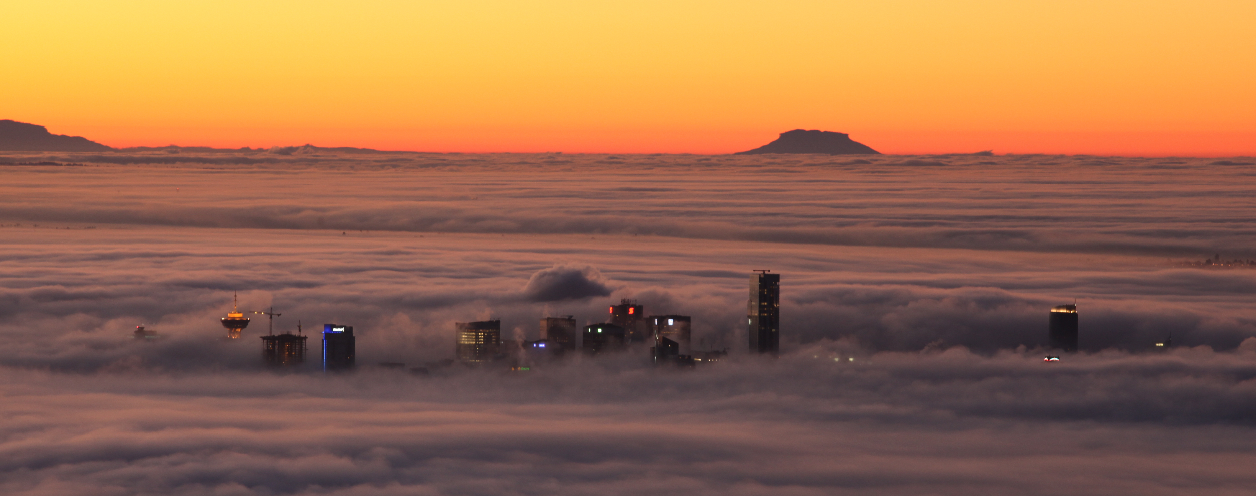
\includegraphics[width=\linewidth, alt={A view of a city with buildings peeking out of the clouds.}]{./assets/imgs/1-cypress-view/cypress-view.jpg}
  \caption{%
  	In the Clouds: Vancouver from Cypress Mountain.
  	Note that the teaser may not be wider than the abstract block.%
  }
  \label{fig:teaser}
}


%% Uncomment below to disable the manuscript note
%\renewcommand{\manuscriptnotetxt}{}

%% Copyright space is enabled by default as required by guidelines.
%% It is disabled by the 'review' option or via the following command:
%\nocopyrightspace


%%%%%%%%%%%%%%%%%%%%%%%%%%%%%%%%%%%%%%%%%%%%%%%%%%%%%%%%%%%%%%%%
%%%%%%%%%%%%%%%%%%%%%% LOAD PACKAGES %%%%%%%%%%%%%%%%%%%%%%%%%%%
%%%%%%%%%%%%%%%%%%%%%%%%%%%%%%%%%%%%%%%%%%%%%%%%%%%%%%%%%%%%%%%%

%% Tell graphicx where to find files for figures when calling \includegraphics.
%% Note that due to the \DeclareGraphicsExtensions{} call it is no longer necessary
%% to provide the the path and extension of a graphics file:
%% 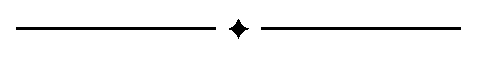
\includegraphics{diamondrule} is completely sufficient.
\graphicspath{{figs/}{figures/}{pictures/}{images/}{./}} % where to search for the images

%% Only used in the template examples. You can remove these lines.
\usepackage{tabu}                      % only used for the table example
\usepackage{booktabs}                  % only used for the table example
\usepackage{lipsum}                    % used to generate placeholder text
\usepackage{mwe}                       % used to generate placeholder figures

%% We encourage the use of mathptmx for consistent usage of times font
%% throughout the proceedings. However, if you encounter conflicts
%% with other math-related packages, you may want to disable it.
\usepackage{mathptmx}                  % use matching math font

\begin{document}

%%%%%%%%%%%%%%%%%%%%%%%%%%%%%%%%%%%%%%%%%%%%%%%%%%%%%%%%%%%%%%%%
%%%%%%%%%%%%%%%%%%%%%% START OF THE PAPER %%%%%%%%%%%%%%%%%%%%%%
%%%%%%%%%%%%%%%%%%%%%%%%%%%%%%%%%%%%%%%%%%%%%%%%%%%%%%%%%%%%%%%%

%% The ``\maketitle'' command must be the first command after the
%% ``\begin{document}'' command. It prepares and prints the title block.
%% the only exception to this rule is the \firstsection command
\maketitle

\section{Introduction}

\revised{Revision is annotated in red.}
\remark{Remark is annotated in brown.}
%% \section{Introduction} %for journal use above \firstsection{..} instead
This template is for papers of VGTC-sponsored conferences such as IEEE VIS, IEEE VR, and ISMAR which are published as special issues of TVCG.
The template does not contain the respective dates of the conference/journal issue, these will be entered by IEEE as part of the publication production process.
Therefore, \textbf{please leave the copyright statement at the bottom-left of this first page untouched}.

\section{Author Details}

You should specify ORCID IDs for each author (see \url{https://orcid.org/}  to register) for disambiguation and long-term contact preservation.
Use \verb|\authororcid{Author Name}{0000-0000-0000-0000}| for each author, replacing the ``Author Name'' and using the 16-digit (hyphenated) ORCID ID for the second parameter.
The template shows an example without ORCID IDs for two of the authors.
ORCID IDs should be provided in all cases.

Each author's affiliations have to be provided in the author footer on the bottom-left corner of the first page.
It is permitted to merge two or more people from the same institution as long as they are shown in the same order as in the overall author sequence on the top of the first page.
For example, if authors A, B, C, and D are from institutions 1, 2, 1, and 2, respectively, then it is ok to use 2 bullets as follows:

\begin{itemize}
  \item A and C are with Institution 1. E-mail: \{a\,$|$\,c\}@i1.com\,.

  \item B and D are with Institution 2. E-mail: \{b\,$|$\,d\}@i2.org\,.
\end{itemize}

\section{Hyperlinks and Cross References}

The style uses the \verb|hyperref| package which can typeset clickable hyperlinks using \verb|\href{...}{...}|, hyperlinked URLs using \verb|\url{...}|, and turns references into internal links.

The style also uses \verb|cleveref| to automatically and consistently format cross references.
We recommend that you use the \verb|\cref{label}| and \verb|\Cref{label}| calls instead of \verb|Figure~\ref{label}| or similar.
\verb|\Cref| should be used when starting a sentence to spell out the reference (e.g.\ ``Section'') while \verb|\cref| should be used when referencing within a sentence to abbreviate (e.g.\ ``Sec.'').
Here are examples for use within a sentence: \cref{fig:vis_papers}, \cref{tab:vis-papers}, \cref{sec:supplement_inst,sec:references_inst}, \cref{eq:sum}.
The following sentences all start with a reference, so use \verb|\Cref|.
\Cref{fig:vis_papers} is a \verb|figure| environment.
\Cref{tab:vis-papers} is a \verb|table| environment.
\Cref{sec:supplement_inst,sec:references_inst} are \verb|section| environments.
\Cref{eq:sum} is an \verb|equation| environment.

\section{Figures}

\subsection{Loading figures}

The style automatically looks for image files with the correct extension (eps for regular \LaTeX; pdf, png, and jpg for pdf\LaTeX), in a set of given subfolders defined above using \verb|\graphicspath|: figures/, pictures/, images/.
It is thus sufficient to use \verb|\includegraphics{CypressView}| (instead of \verb|\includegraphics{pictures/CypressView.jpg}|).
Figures should be in CMYK or Grey scale format, otherwise, colour shifting may occur during the printing process.

\subsection{Vector figures}

Vector graphics like svg, eps, pdf are best for charts and other figures with text or lines.
They will look much nicer and crisper and any text in them will be more selectable, searchable, and accessible.

\subsection{Raster figures}

Of the raster graphics formats, screenshots of user interfaces and text, as well as line art, are better shown with png.
jpg is better for photographs.
Make sure all raster graphics are captured in high enough resolution so they look crisp and scale well.

\subsection{Alt texts}

Add alternative texts that describe the content of the image to all figures.

\subsection{Figures on the first page}

The teaser figure should only have the width of the abstract as the template enforces it.
The use of figures other than the optional teaser is not permitted on the first page.
Other figures should begin on the second page.
Papers submitted with figures other than the optional teaser on the first page will be refused.

\subsection{Subfigures}

You can add subfigures using the \texttt{subcaption} package that is automatically loaded.
Inside a \verb|figure| environment, create a \verb|subfigure| environment.
See \cref{fig:ex_subfigs} for an example.
You can reference individual figures, either fully using \verb|\cref| (\cref{fig:ex_subfigs_a,fig:ex_subfigs_b}) or by letter using \verb|\subref|.
E.g., \subref{fig:ex_subfigs_b}, \subref{fig:ex_subfigs_c}.
Note that \verb|\subref| only works for one label at a time.

\begin{figure}[tbp]
  \centering
  \begin{subfigure}[b]{0.45\columnwidth}
  	\centering
  	\includegraphics[width=\textwidth, alt={Big letter A on a gray background.}]{example-image-a}
  	\caption{The letter A.}
  	\label{fig:ex_subfigs_a}
  \end{subfigure}%
  \hfill%
  \begin{subfigure}[b]{0.45\columnwidth}
  	\centering
  	\includegraphics[width=\textwidth, alt={Big letter B on a gray background.}]{example-image-b}
  	\caption{The letter B.}
  	\label{fig:ex_subfigs_b}
  \end{subfigure}%
  \\%
  \begin{subfigure}[b]{0.45\columnwidth}
  	\centering
  	\includegraphics[width=\textwidth, alt={Big letter C on a gray background.}]{example-image-c}
  	\caption{The letter C.}
  	\label{fig:ex_subfigs_c}
  \end{subfigure}%
  \subfigsCaption{Example of adding subfigures with the \texttt{subcaption} package.}
  \label{fig:ex_subfigs}
\end{figure}

\subsection{Figure Credits}
\label{sec:figure_credits_inst}

In the \hyperref[sec:figure_credits]{Figure Credits} section at the end of the paper, you should credit the original sources of any figures that were reproduced or modified.
Include any license details necessary, as well as links to the original materials whenever possible.
For credits to figures from academic papers, include a citation that is listed in the \textbf{References} section.
An example is provided \hyperref[sec:figure_credits]{below}.

\section{Equations and Tables}

Equations can be added like so:

\begin{equation}
  \label{eq:sum}
  \sum_{j=1}^{z} j = \frac{z(z+1)}{2}
\end{equation}

Tables, such as \cref{tab:vis-papers} can also be included.

\begin{table}[tb]
  \caption{%
    VIS/VisWeek accepted/presented papers: 1990--2016.%
  }
  \label{tab:vis-papers}
  \scriptsize%
  \centering%
  \begin{tabu}{%
      r%
        *{7}{c}%
        *{2}{r}%
    }
    \toprule
    year         & \rotatebox{90}{Vis/SciVis} & \rotatebox{90}{SciVis conf} & \rotatebox{90}{InfoVis} & \rotatebox{90}{VAST} & \rotatebox{90}{VAST conf} & \rotatebox{90}{TVCG @ VIS} & \rotatebox{90}{CG\&A @ VIS} & \rotatebox{90}{VIS/VisWeek} \rotatebox{90}{incl.\ TVCG/CG\&A} & \rotatebox{90}{VIS/VisWeek} \rotatebox{90}{w/o TVCG/CG\&A} \\
    \midrule
    2016         & 30                         &                             & 37                      & 33                   & 15                        & 23                         & 10                          & 148                                                           & 115                                                        \\
    2015         & 33                         & 9                           & 38                      & 33                   & 14                        & 17                         & 15                          & 159                                                           & 127                                                        \\
    2014         & 34                         &                             & 45                      & 33                   & 21                        & 20                         &                             & 153                                                           & 133                                                        \\
    2013         & 31                         &                             & 38                      & 32                   &                           & 20                         &                             & 121                                                           & 101                                                        \\
    2012         & 42                         &                             & 44                      & 30                   &                           & 23                         &                             & 139                                                           & 116                                                        \\
    2011         & 49                         &                             & 44                      & 26                   &                           & 20                         &                             & 139                                                           & 119                                                        \\
    2010         & 48                         &                             & 35                      & 26                   &                           &                            &                             & 109                                                           & 109                                                        \\
    2009         & 54                         &                             & 37                      & 26                   &                           &                            &                             & 117                                                           & 117                                                        \\
    2008         & 50                         &                             & 28                      & 21                   &                           &                            &                             & 99                                                            & 99                                                         \\
    2007         & 56                         &                             & 27                      & 24                   &                           &                            &                             & 107                                                           & 107                                                        \\
    2006         & 63                         &                             & 24                      & 26                   &                           &                            &                             & 113                                                           & 113                                                        \\
    2005         & 88                         &                             & 31                      &                      &                           &                            &                             & 119                                                           & 119                                                        \\
    2004         & 70                         &                             & 27                      &                      &                           &                            &                             & 97                                                            & 97                                                         \\
    2003         & 74                         &                             & 29                      &                      &                           &                            &                             & 103                                                           & 103                                                        \\
    2002         & 78                         &                             & 23                      &                      &                           &                            &                             & 101                                                           & 101                                                        \\
    2001         & 74                         &                             & 22                      &                      &                           &                            &                             & 96                                                            & 96                                                         \\
    2000         & 73                         &                             & 20                      &                      &                           &                            &                             & 93                                                            & 93                                                         \\
    1999         & 69                         &                             & 19                      &                      &                           &                            &                             & 88                                                            & 88                                                         \\
    1998         & 72                         &                             & 18                      &                      &                           &                            &                             & 90                                                            & 90                                                         \\
    1997         & 72                         &                             & 16                      &                      &                           &                            &                             & 88                                                            & 88                                                         \\
    1996         & 65                         &                             & 12                      &                      &                           &                            &                             & 77                                                            & 77                                                         \\
    1995         & 56                         &                             & 18                      &                      &                           &                            &                             & 74                                                            & 74                                                         \\
    1994         & 53                         &                             &                         &                      &                           &                            &                             & 53                                                            & 53                                                         \\
    1993         & 55                         &                             &                         &                      &                           &                            &                             & 55                                                            & 55                                                         \\
    1992         & 53                         &                             &                         &                      &                           &                            &                             & 53                                                            & 53                                                         \\
    1991         & 50                         &                             &                         &                      &                           &                            &                             & 50                                                            & 50                                                         \\
    1990         & 53                         &                             &                         &                      &                           &                            &                             & 53                                                            & 53                                                         \\
    \midrule
    \textbf{sum} & \textbf{1545}              & \textbf{9}                  & \textbf{632}            & \textbf{310}         & \textbf{50}               & \textbf{123}               & \textbf{25}                 & \textbf{2694}                                                 & \textbf{2546}                                              \\
    \bottomrule
  \end{tabu}%
\end{table}


\begin{figure}[tb]% specify a combination of t, b, p, or h for top, bottom, on its own page, or here
  \centering % avoid the use of \begin{center}...\end{center} and use \centering instead (more compact)
  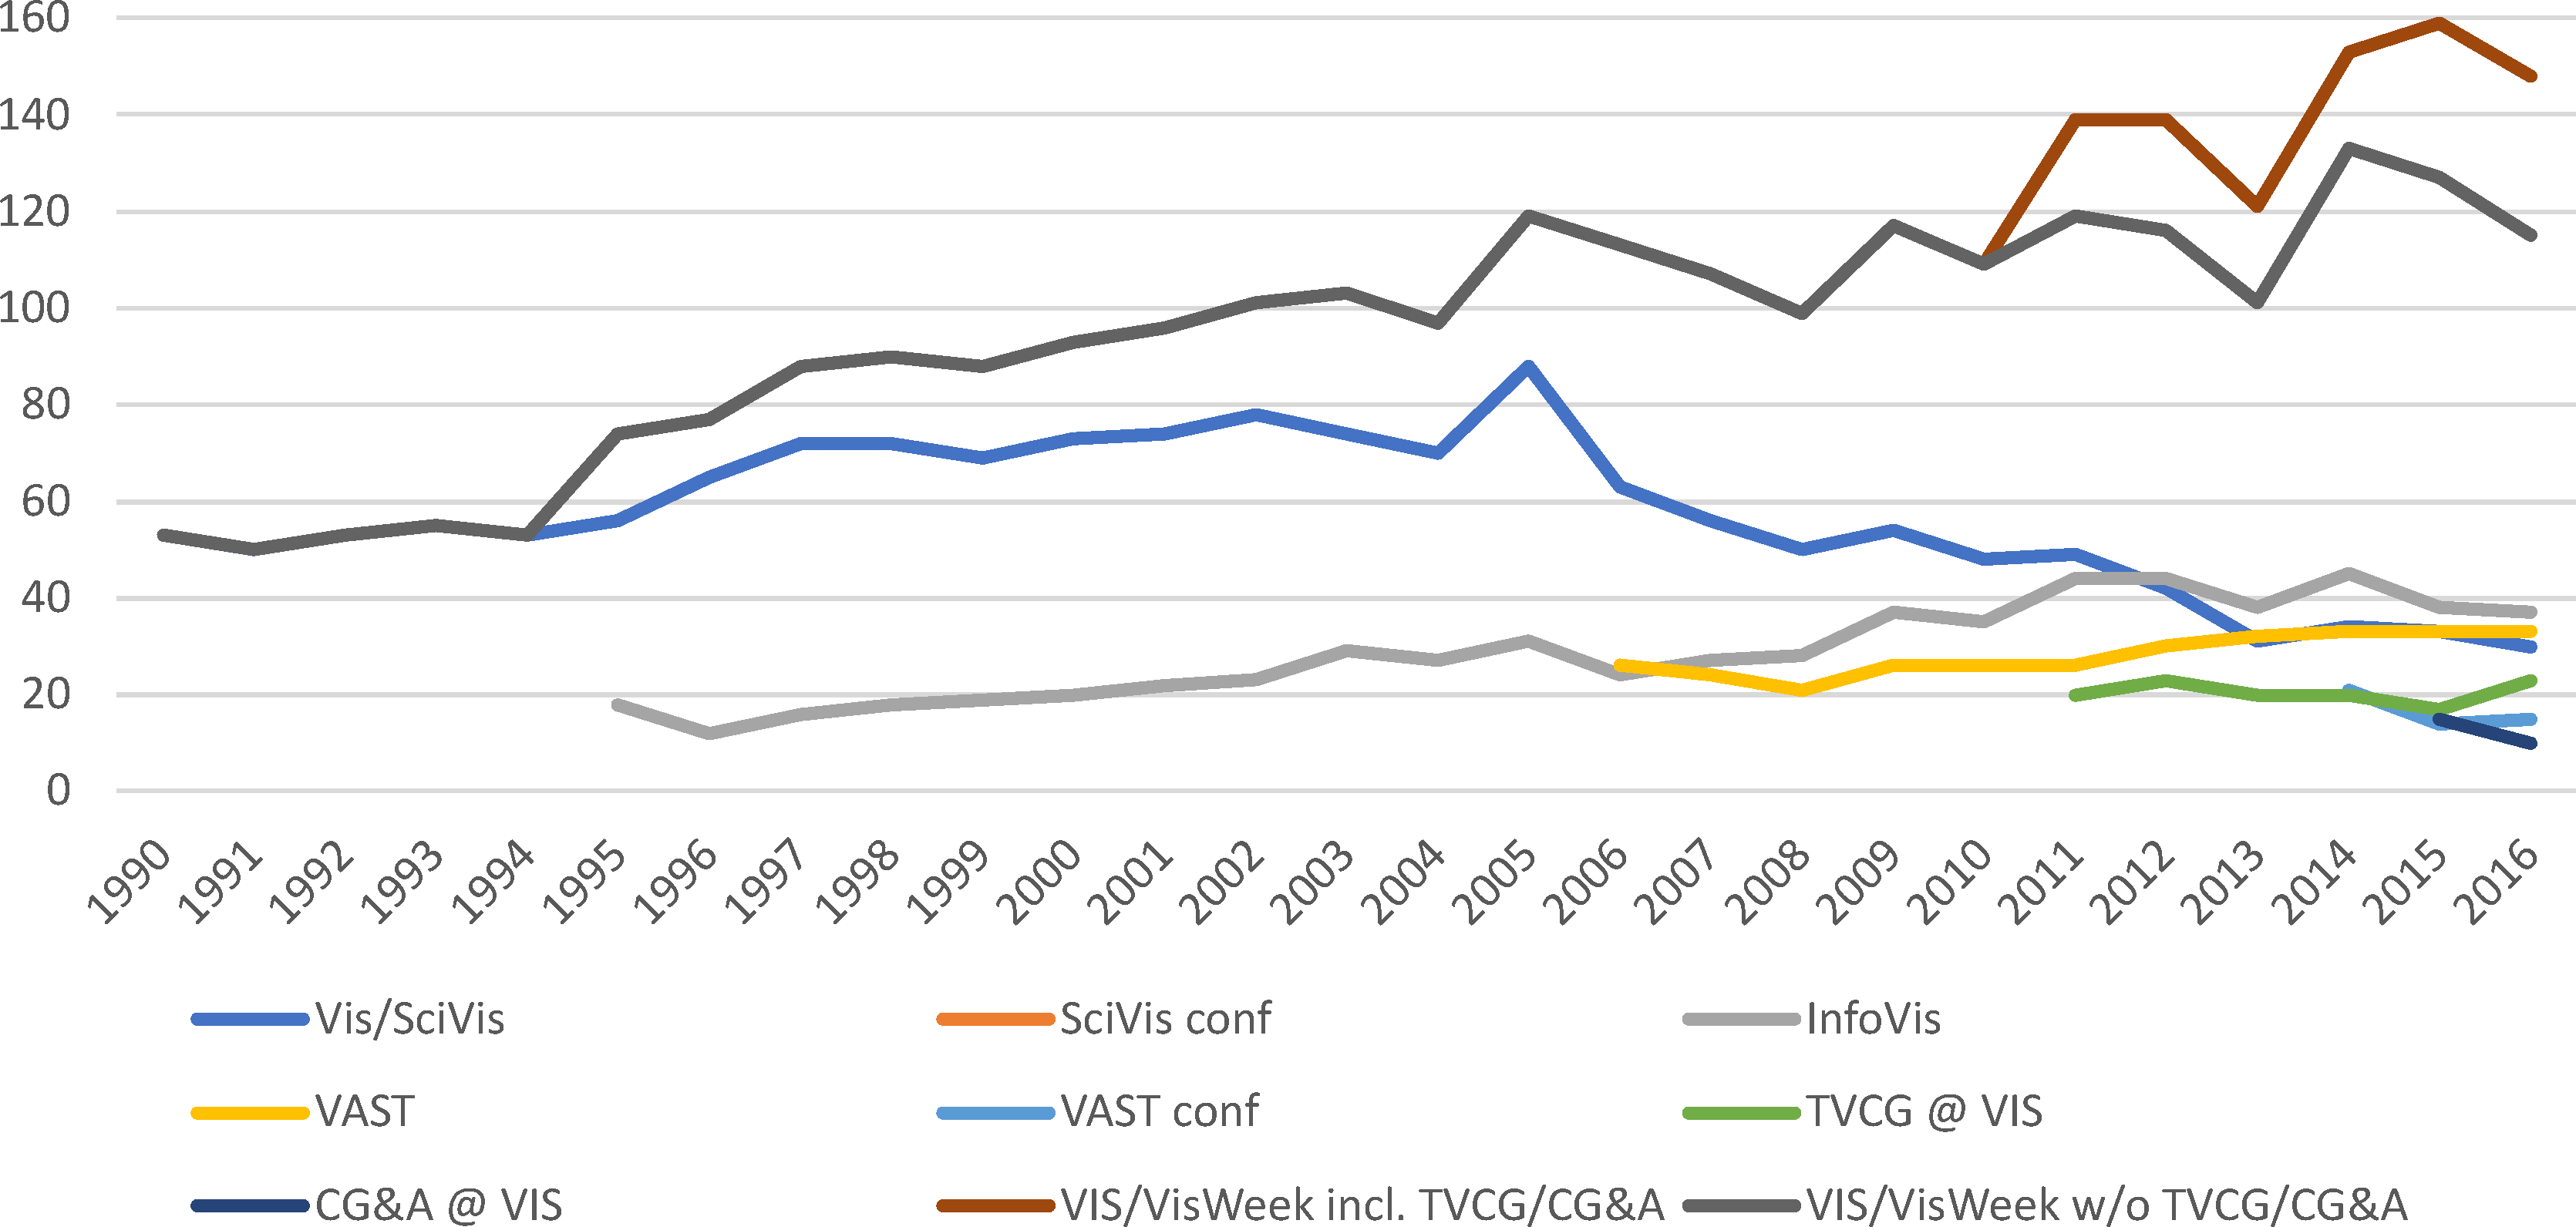
\includegraphics[width=\columnwidth, alt={A line graph showing paper counts between 0 and 160 from 1990 to 2016 for 9 venues.}]{./assets/imgs/2-paper-count-2016/paper-count-2016.pdf}
  \caption{%
  	A visualization of the 1990--2016 data from \cref{tab:vis-papers}, recreated based on Fig.\ 1 from \cite{Isenberg2017Vispubdata.orgMetadataCollection}.%
  }
  \label{fig:vis_papers}
\end{figure}

\section{Supplemental Material Instructions}
\label{sec:supplement_inst}

In support of transparent research practices and long-term open science goals, you are encouraged to make your supplemental materials available on a publicly-accessible repository.
Please describe the available supplemental materials in the \hyperref[sec:supplemental_materials]{Supplemental Materials} section.
These details could include (1) what materials are available, (2) where they are hosted, and (3) any necessary omissions.

\section{Appendices}
\label{sec:appendices_inst}

Appendices can be specified using \verb|\appendix|.
For example, our Troubleshooting instructions in
\iflabelexists{appendix:troubleshooting}
  {\cref{appendix:troubleshooting}}
  {the appendix of the full paper at \url{https://osf.io/nrmyc}}.

Note that the paper submission has to end after the \textbf{References} section and within the page limit of the conference you are submitting to.
Any version of Appendices or the paper with Appendices included has to be submitted separately as supplementary material.
You can use the \verb|hideappendix| class option to remove everything after \verb|\appendix|.
We encourage you to submit a full version of your paper to a preprint server with any appendices included.

You can use the \verb|\iflabelexists| macro to cross reference an appendix from the main text, but only if that label (i.e.\ the appendix) actually exists.
For example, above we use 

\begin{verbatim}
\iflabelexists{appendix:troubleshooting}
  {\cref{appendix:troubleshooting}}
  {the appendix of the full paper at
   \url{https://osf.io/XXXXX}}.
\end{verbatim}

in order to cross-reference to the appendix with \verb|\cref| if it exists, but if the appendix is commented out then we will simply create a hyperlinked URL to it.

\section{References}
\label{sec:references_inst}

An example of the reference formatting is provided in the \textbf{References} section at the end.

\subsection{Include DOIs}

All references which have a DOI should have it included in the bib\TeX\ for the style to display.
The DOI can be entered with or without the \url{https://doi.org/} prefix.

\subsection{Narrow DOI option}

The \verb|-narrow| versions of the bibliography style use the font \verb|PTSansNarrow-TLF| for typesetting the DOIs in a compact way.
This font needs to be available on your \LaTeX\ system.
It is part of the \href{https://www.ctan.org/pkg/paratype}{\texttt{paratype} package}, and many distributions (such as MikTeX) have it automatically installed.
If you do not have this package yet and want to use a \verb|-narrow| bibliography style then use your \LaTeX\ system's package installer to add it.
If this is not possible you can also revert to the respective bibliography styles without the \verb|-narrow| in the file name.
DVI-based processes to compile the template apparently cannot handle the different font so, by default, the template file uses the \texttt{abbrv-doi} bibliography style.

\subsection{Disabling hyperlinks}

To avoid adding hyperlinks to the references (the default) you can use \verb|\bibliographystyle{abbrv-doi}| instead of \verb|\bibliographystyle{abbrv-doi-hyperref}|.
By default, the DOI field in a bib\TeX\ entry is turned into a hyperlink.

See the examples in the bib\TeX\ file and the bibliography at the end of this template.

\subsection{Guidelines for bibTeX}

\begin{itemize}
  \item All bibliographic entries should be sorted alphabetically by the last name of the first author.
        This \LaTeX/bib\TeX\ template takes care of this sorting automatically.
  \item Merge multiple references into one; e.\,g., use \cite{Max1995OpticalModelsDirect,Kitware2003VisualizationToolkitUsers} (not \cite{Kitware2003VisualizationToolkitUsers}\cite{Max1995OpticalModelsDirect}).
        Within each set of multiple references, the references should be sorted in ascending order.
        This \LaTeX/bib\TeX\ template takes care of both the merging and the sorting automatically.
  \item Verify all data obtained from digital libraries, even ACM's DL and IEEE Xplore  etc.\ are sometimes wrong or incomplete.
  \item Do not trust bibliographic data from other services such as Mendeley.com, Google Scholar, or similar; these are even more likely to be incorrect or incomplete.
  \item Articles in journal---items to include:
        \begin{itemize}
          \item author names
          \item title
          \item journal name
          \item year
          \item volume
          \item number
          \item month of publication as variable name (i.e., \{jan\} for January, etc.; month ranges using \{jan \#\{/\}\# feb\} or \{jan \#\{-{}-\}\# feb\})
          \item series. E.g., ``TVCG``, ``TVCG/VIS`` for special issue VIS papers, ``EuroVis``, ``CGF/EuroVis``.
        \end{itemize}
  \item Use journal names in proper style: correct: ``IEEE Transactions on Visualization and Computer Graphics'', incorrect: ``Visualization and Computer Graphics, IEEE Transactions on''
  \item Papers in proceedings---items to include:
        \begin{itemize}
          \item author names
          \item title
          \item abbreviated proceedings name: e.g., ``Proc.\textbackslash{} CONF\_ACRONYNM'' without the year; example: ``Proc.\textbackslash{} CHI'', ``Proc.\textbackslash{} 3DUI'', ``Proc.\textbackslash{} Eurographics'', ``Proc.\textbackslash{} EuroVis''
          \item year
          \item series. E.g., ``VIS`` and ``EuroVis`` for short papers, ``CHI``...
        \end{itemize}

  \item Article/paper title convention: refrain from using curly brackets, except for acronyms/proper names/words following dashes/question marks etc.; example:\\\\
        %
        The paper ``Marching Cubes: A High Resolution 3D Surface Construction Algorithm'' should be entered as ``\{M\}arching \{C\}ubes: A High Resolution \{3D\} Surface Construction Algorithm'' or  ``\{M\}arching \{C\}ubes: A high resolution \{3D\} surface construction algorithm''.
        It will then be typeset as ``Marching Cubes: A high resolution 3D surface construction algorithm''.
  \item For all entries:
        \begin{itemize}
          \item DOI can be entered in the DOI field as plain DOI number or as DOI url.
          \item ``pages`` or ``articleno``: Provide full page ranges AA-{}-BB, OR, if an article number is available like recent ACM conferences, use that instead. E.g., see the entry for Panavas et al.\ \cite{Panavas2022JuvenileGraphicalPerception}.
        \end{itemize}
  \item When citing references, do not use the reference as a sentence object; e.g., wrong: ``In \cite{Lorensen1987MarchingCubesHigh} the authors describe \dots'', correct: ``Lorensen and Cline \cite{Lorensen1987MarchingCubesHigh} describe \dots''
\end{itemize}

\section{Filler Text to Flush Out the Paper}

\lipsum[1-2]% Just add some more arbitrary text so we see a fuller paper example


\section*{Supplemental Materials}
\label{sec:supplemental_materials}

Refer to the instructions for this section (\cref{sec:supplement_inst}).
Below is an example you can follow that includes the actual supplemental material for this template:

All supplemental materials are available on OSF at \url{https://doi.org/10.17605/OSF.IO/2NBSG}, released under a CC BY 4.0 license.
In particular, they include (1) Excel files containing the data for and analyses for creating \cref{tab:vis-papers} and \cref{fig:vis_papers}, (2) figure images in multiple formats, and (3) a full version of this paper with all appendices.
Our other code is intellectual property of a corporation---Starbucks Research---and there is no feasible way to share it publicly.

\section*{Figure Credits}
\label{sec:figure_credits}

Refer to the instructions for this section (\cref{sec:figure_credits_inst}).
Here are the actual figure credits for this template:

\Cref{fig:teaser} image credit: Scott Miller / Special to the Vancouver Sun, January 22, 2009, page A6.

\Cref{fig:vis_papers} is a partial recreation of Fig.\ 1 from \cite{Isenberg2017Vispubdata.orgMetadataCollection}, which is in the public domain.


%% if specified like this the section will be omitted in review mode
\acknowledgments{%
  The authors wish to thank A, B, and C.
This work was supported in part by a grant from XYZ (\# 12345-67890).%

}

\bibliographystyle{abbrv-doi-hyperref}
%\bibliographystyle{abbrv-doi-hyperref-narrow}
%\bibliographystyle{abbrv-doi}
%\bibliographystyle{abbrv-doi-narrow}

\bibliography{assets/bibs/papers.bib}

\appendix % You can use the `hideappendix` class option to skip everything after \appendix

\section{About Appendices}

Refer to \cref{sec:appendices_inst} for instructions regarding appendices.

\section{Troubleshooting}
\label{appendix:troubleshooting}

\subsection{ifpdf error}

If you receive compilation errors along the lines of \texttt{Package ifpdf Error: Name clash, \textbackslash ifpdf is already defined} then please add a new line \verb|\let\ifpdf\relax| right after the \verb|\documentclass[journal]{vgtc}| call.
Note that your error is due to packages you use that define \verb|\ifpdf| which is obsolete (the result is that \verb|\ifpdf| is defined twice); these packages should be changed to use \verb|ifpdf| package instead.

\subsection{\texttt{pdfendlink} error}

Occasionally (for some \LaTeX\ distributions) this hyper-linked bib\TeX\ style may lead to \textbf{compilation errors} (\texttt{pdfendlink ended up in different nesting level ...}) if a reference entry is broken across two pages (due to a bug in \verb|hyperref|).
In this case, make sure you have the latest version of the \verb|hyperref| package (i.e.\ update your \LaTeX\ installation/packages) or, alternatively, revert back to \verb|\bibliographystyle{abbrv-doi}| (at the expense of removing hyperlinks from the bibliography) and try \verb|\bibliographystyle{abbrv-doi-hyperref}| again after some more editing.


\end{document}
